\documentclass[a4paper,12pt]{article}
\usepackage[margin=1in]{geometry}
\usepackage{graphicx}
\usepackage{fancyhdr}
\usepackage{setspace}
\usepackage{titlesec}
\usepackage{longtable}
\usepackage{array}
\usepackage{caption}
\usepackage{amsmath}
\usepackage{amssymb}
\usepackage{listings}
\usepackage{xcolor}
\usepackage{hyperref}

% Code listing style
\lstdefinestyle{pythonstyle}{
    language=Python,
    basicstyle=\ttfamily\footnotesize,
    keywordstyle=\color{blue}\bfseries,
    stringstyle=\color{red},
    commentstyle=\color{green!60!black},
    numbers=left,
    numberstyle=\tiny\color{gray},
    numbersep=5pt,
    breaklines=true,
    showstringspaces=false,
    frame=single,
    backgroundcolor=\color{gray!10},
    tabsize=4
}

% Page number bottom center
\pagestyle{fancy}
\fancyhf{}
\fancyfoot[C]{\thepage}
\renewcommand{\headrulewidth}{0pt}

\begin{document}

% ----------------- Title Page -----------------
\begin{titlepage}
    \centering
    {\Large \textbf{National University of Modern Languages, Islamabad}} \par
    \vspace{2cm}
    {\Huge \bfseries Speech Processing Lab Report \par}
    \vspace{2cm}
    {\Large \textit{Final Project: Real-Time Speech Recognition System} \par}
    \vspace{0.5cm}
    {\large \textit{Recognizing Spoken Digits Using CNN and MFCC Features} \par}
    \vspace{3cm}
    {\large \textbf{Submitted by:} \\ Junaid Asif} \par
    \vspace{0.3cm}
    {\large \textbf{Roll No:} BSAI-144} \par
    \vspace{0.3cm}
    {\large \textbf{Instructor:} Dr. Sajjad Ghauri} \par
    \vfill
    {\large December 23, 2025}
\end{titlepage}

\setstretch{1.2}

% ----------------- Table of Contents -----------------
\tableofcontents
\newpage

% ----------------- Objective -----------------
\section{Objective}
The objective of this project is to design and implement a Python-based system that can recognize a small set of predefined speech commands (spoken digits from ``zero'' to ``nine'') in real-time from a live microphone audio stream, displaying the recognized command with minimal latency.

\subsection{Specific Goals}
\begin{itemize}
    \item Create a custom dataset by recording isolated spoken digits.
    \item Extract MFCC (Mel-Frequency Cepstral Coefficients) features along with delta and delta-delta coefficients.
    \item Train a Convolutional Neural Network (CNN) for speech classification.
    \item Implement real-time Voice Activity Detection (VAD).
    \item Build a live recognition system with confidence-based output.
\end{itemize}

% ----------------- Theoretical Background -----------------
\section{Theoretical Background}

\subsection{Real-Time Audio Processing}
Real-time audio processing involves capturing, analyzing, and responding to audio signals with minimal delay. The system uses a sliding buffer approach where audio is continuously captured from the microphone and processed in fixed-duration windows.

\subsection{Mel-Frequency Cepstral Coefficients (MFCCs)}
MFCCs are widely used features in speech and audio processing that represent the short-term power spectrum of sound. The extraction process involves:

\begin{enumerate}
    \item \textbf{Pre-emphasis:} Boosting high frequencies to balance the spectrum.
    \item \textbf{Framing:} Dividing the signal into short overlapping frames.
    \item \textbf{Windowing:} Applying a Hamming window to each frame.
    \item \textbf{FFT:} Computing the Fast Fourier Transform.
    \item \textbf{Mel Filter Bank:} Applying triangular filters on a mel scale.
    \item \textbf{Log Compression:} Taking the logarithm of filter bank energies.
    \item \textbf{DCT:} Applying Discrete Cosine Transform to get MFCCs.
\end{enumerate}

The mel scale converts frequency $f$ (Hz) to mel scale $m$ using:
\begin{equation}
    m = 2595 \cdot \log_{10}\left(1 + \frac{f}{700}\right)
\end{equation}

\subsection{Delta and Delta-Delta Coefficients}
To capture temporal dynamics, we compute:
\begin{itemize}
    \item \textbf{Delta (Velocity):} First-order derivative of MFCCs
    \item \textbf{Delta-Delta (Acceleration):} Second-order derivative of MFCCs
\end{itemize}

The delta coefficient is computed as:
\begin{equation}
    \Delta c_t = \frac{\sum_{n=1}^{N} n(c_{t+n} - c_{t-n})}{2\sum_{n=1}^{N} n^2}
\end{equation}

\subsection{Convolutional Neural Networks (CNNs)}
CNNs are deep learning models effective for pattern recognition in structured data. For speech recognition, the MFCC features are treated as 2D images where:
\begin{itemize}
    \item \textbf{Height:} Number of MFCC coefficients (39 = 13 × 3)
    \item \textbf{Width:} Number of time frames
    \item \textbf{Channels:} 1 (grayscale representation)
\end{itemize}

\subsection{Voice Activity Detection (VAD)}
VAD determines whether a given audio segment contains speech or silence. We use Root Mean Square (RMS) energy:
\begin{equation}
    RMS = \sqrt{\frac{1}{n}\sum_{i=1}^{n} x_i^2}
\end{equation}
If $RMS > \text{threshold}$, speech is detected.

% ----------------- Tools and Libraries -----------------
\section{Tools and Libraries}

\subsection{Software Requirements}
\begin{itemize}
    \item \textbf{Python 3.10+} - Programming language
    \item \textbf{TensorFlow/Keras} - Deep learning framework
    \item \textbf{Librosa} - Audio analysis and feature extraction
    \item \textbf{NumPy} - Numerical computing
    \item \textbf{SciPy} - Scientific computing
    \item \textbf{Sounddevice} - Real-time audio recording
    \item \textbf{Soundfile} - Audio file I/O
    \item \textbf{Scikit-learn} - Machine learning utilities
    \item \textbf{Matplotlib} - Visualization
\end{itemize}

\subsection{Hardware Requirements}
\begin{itemize}
    \item Working microphone connected to the computer
    \item Minimum 4GB RAM
    \item CPU with AVX support (for TensorFlow)
\end{itemize}

% ----------------- System Architecture -----------------
\section{System Architecture}

\subsection{Project Structure}
\begin{verbatim}
speech_recognition/
├── venv/                      # Virtual environment
├── dataset/                   # Recorded audio samples
│   ├── zero/
│   ├── one/
│   └── ... (nine/)
├── models/                    # Trained models
│   ├── speech_recognition_model.keras
│   ├── normalization_params.npy
│   └── label_map.npy
├── config.py                  # Configuration settings
├── record_dataset.py          # Dataset recording
├── feature_extraction.py      # MFCC extraction
├── train_model.py             # CNN training
├── realtime_recognition.py    # Live recognition
└── main.py                    # Main interface
\end{verbatim}

\subsection{System Flow Diagram}
\begin{center}
\begin{tabular}{|c|}
\hline
\textbf{Audio Input (Microphone)} \\
\hline
$\downarrow$ \\
\hline
\textbf{Voice Activity Detection} \\
\hline
$\downarrow$ \\
\hline
\textbf{MFCC Feature Extraction} \\
\hline
$\downarrow$ \\
\hline
\textbf{Feature Normalization} \\
\hline
$\downarrow$ \\
\hline
\textbf{CNN Model Inference} \\
\hline
$\downarrow$ \\
\hline
\textbf{Prediction + Confidence} \\
\hline
\end{tabular}
\end{center}

% ----------------- Configuration -----------------
\section{Configuration Settings}

\subsection{Audio Parameters}
\begin{lstlisting}[style=pythonstyle]
# Audio Settings
SAMPLE_RATE = 16000  # 16 kHz sampling rate
DURATION = 1.0       # 1 second recording duration
CHANNELS = 1         # Mono audio
\end{lstlisting}

\subsection{Feature Extraction Parameters}
\begin{lstlisting}[style=pythonstyle]
# MFCC Feature Settings
N_MFCC = 13          # Number of MFCC coefficients
N_FFT = 512          # FFT window size
HOP_LENGTH = 160     # Hop length (10ms at 16kHz)
N_MELS = 40          # Number of mel bands
\end{lstlisting}

\textbf{Explanation of Parameters:}
\begin{itemize}
    \item \textbf{N\_MFCC = 13:} Standard number of coefficients capturing vocal tract shape.
    \item \textbf{N\_FFT = 512:} FFT window size (~32ms at 16kHz).
    \item \textbf{HOP\_LENGTH = 160:} Frame shift of 10ms for smooth temporal resolution.
    \item \textbf{N\_MELS = 40:} Number of mel filter banks.
\end{itemize}

\subsection{Training Parameters}
\begin{lstlisting}[style=pythonstyle]
# Training Settings
BATCH_SIZE = 32
EPOCHS = 50
VALIDATION_SPLIT = 0.2
LEARNING_RATE = 0.001
\end{lstlisting}

\subsection{Recognition Parameters}
\begin{lstlisting}[style=pythonstyle]
# Real-time Recognition Settings
CONFIDENCE_THRESHOLD = 0.6  # Minimum 60% confidence
SILENCE_THRESHOLD = 0.01    # RMS threshold for VAD
BUFFER_DURATION = 1.0       # 1 second audio buffer
\end{lstlisting}

% ----------------- Dataset Recording -----------------
\section{Dataset Recording}

\subsection{Recording Script}
The dataset consists of isolated spoken digits from ``zero'' to ``nine'', recorded multiple times for training diversity.

\begin{lstlisting}[style=pythonstyle]
import sounddevice as sd
import soundfile as sf
import numpy as np

def record_audio(duration=1.0, sample_rate=16000):
    """Record audio from microphone."""
    print("Recording...", end=" ", flush=True)
    audio = sd.rec(int(duration * sample_rate), 
                   samplerate=sample_rate, 
                   channels=1, 
                   dtype='float32')
    sd.wait()  # Wait for recording to complete
    print("Done!")
    return audio.flatten()

def save_audio(audio, filepath, sample_rate=16000):
    """Save audio to WAV file."""
    sf.write(filepath, audio, sample_rate)
\end{lstlisting}

\subsection{Dataset Specifications}
\begin{table}[h]
\centering
\begin{tabular}{|l|l|}
\hline
\textbf{Parameter} & \textbf{Value} \\
\hline
Classes & zero, one, two, ..., nine (10 classes) \\
\hline
Recordings per class & 3-10 samples \\
\hline
Sample rate & 16,000 Hz \\
\hline
Duration & 1 second per recording \\
\hline
Format & WAV (mono) \\
\hline
\end{tabular}
\caption{Dataset Specifications}
\end{table}

% ----------------- Feature Extraction -----------------
\section{Feature Extraction}

\subsection{MFCC Extraction Code}
\begin{lstlisting}[style=pythonstyle]
import librosa
import numpy as np

def extract_mfcc_features(audio, sample_rate=16000, n_mfcc=13, 
                          n_fft=512, hop_length=160, n_mels=40):
    """
    Extract MFCC features with delta and delta-delta.
    Returns: Stacked features (39, time_frames)
    """
    # Extract MFCCs
    mfccs = librosa.feature.mfcc(
        y=audio, sr=sample_rate, n_mfcc=n_mfcc,
        n_fft=n_fft, hop_length=hop_length, n_mels=n_mels
    )
    
    # Compute delta (first derivative)
    delta_mfccs = librosa.feature.delta(mfccs)
    
    # Compute delta-delta (second derivative)
    delta2_mfccs = librosa.feature.delta(mfccs, order=2)
    
    # Stack all features: (39, time_frames)
    features = np.vstack([mfccs, delta_mfccs, delta2_mfccs])
    
    return features
\end{lstlisting}

\subsection{Feature Dimensions}
For a 1-second audio at 16kHz with hop length of 160:
\begin{itemize}
    \item Number of frames: $\lceil 16000 / 160 \rceil + 1 = 101$
    \item MFCC coefficients: 13
    \item With deltas: $13 \times 3 = 39$
    \item Final shape: $(39, 101, 1)$
\end{itemize}

\subsection{Normalization}
Z-score normalization is applied to standardize features:
\begin{equation}
    X_{normalized} = \frac{X - \mu}{\sigma + \epsilon}
\end{equation}
where $\mu$ is the mean, $\sigma$ is the standard deviation, and $\epsilon = 10^{-8}$ prevents division by zero.

% ----------------- CNN Model -----------------
\section{CNN Model Architecture}

\subsection{Model Design}
\begin{lstlisting}[style=pythonstyle]
from tensorflow.keras import layers, models

def create_cnn_model(input_shape, num_classes):
    model = models.Sequential([
        layers.Input(shape=input_shape),
        
        # Block 1
        layers.Conv2D(32, (3, 3), padding='same'),
        layers.BatchNormalization(),
        layers.Activation('relu'),
        layers.MaxPooling2D((2, 2)),
        layers.Dropout(0.25),
        
        # Block 2
        layers.Conv2D(64, (3, 3), padding='same'),
        layers.BatchNormalization(),
        layers.Activation('relu'),
        layers.MaxPooling2D((2, 2)),
        layers.Dropout(0.25),
        
        # Block 3
        layers.Conv2D(128, (3, 3), padding='same'),
        layers.BatchNormalization(),
        layers.Activation('relu'),
        layers.MaxPooling2D((2, 2)),
        layers.Dropout(0.25),
        
        # Block 4
        layers.Conv2D(256, (3, 3), padding='same'),
        layers.BatchNormalization(),
        layers.Activation('relu'),
        
        # Global Pooling
        layers.GlobalAveragePooling2D(),
        
        # Dense Layers
        layers.Dense(128),
        layers.BatchNormalization(),
        layers.Activation('relu'),
        layers.Dropout(0.5),
        
        layers.Dense(64),
        layers.BatchNormalization(),
        layers.Activation('relu'),
        layers.Dropout(0.5),
        
        # Output
        layers.Dense(num_classes, activation='softmax')
    ])
    
    model.compile(
        optimizer='adam',
        loss='sparse_categorical_crossentropy',
        metrics=['accuracy']
    )
    return model
\end{lstlisting}

\subsection{Architecture Summary}
\begin{table}[h]
\centering
\begin{tabular}{|l|l|l|}
\hline
\textbf{Layer} & \textbf{Output Shape} & \textbf{Parameters} \\
\hline
Input & (39, 101, 1) & 0 \\
\hline
Conv2D + BN + ReLU + Pool & (19, 50, 32) & 320 \\
\hline
Conv2D + BN + ReLU + Pool & (9, 25, 64) & 18,496 \\
\hline
Conv2D + BN + ReLU + Pool & (4, 12, 128) & 73,856 \\
\hline
Conv2D + BN + ReLU & (4, 12, 256) & 295,168 \\
\hline
GlobalAveragePooling2D & (256) & 0 \\
\hline
Dense + BN + ReLU & (128) & 33,024 \\
\hline
Dense + BN + ReLU & (64) & 8,320 \\
\hline
Dense (Softmax) & (10) & 650 \\
\hline
\textbf{Total} & & \textbf{~430,000} \\
\hline
\end{tabular}
\caption{CNN Architecture Summary}
\end{table}

\subsection{Training Process}
\begin{lstlisting}[style=pythonstyle]
# Callbacks for training
callbacks = [
    EarlyStopping(
        monitor='val_loss',
        patience=10,
        restore_best_weights=True
    ),
    ReduceLROnPlateau(
        monitor='val_loss',
        factor=0.5,
        patience=5,
        min_lr=1e-6
    ),
    ModelCheckpoint(
        'models/speech_recognition_model.keras',
        monitor='val_accuracy',
        save_best_only=True
    )
]

# Train
history = model.fit(
    X_train, y_train,
    batch_size=32,
    epochs=50,
    validation_data=(X_test, y_test),
    callbacks=callbacks
)
\end{lstlisting}

% ----------------- Real-Time Recognition -----------------
\section{Real-Time Recognition System}

\subsection{Voice Activity Detection}
\begin{lstlisting}[style=pythonstyle]
def compute_rms(audio):
    """Compute Root Mean Square energy."""
    return np.sqrt(np.mean(audio**2))

def is_speech(audio, threshold=0.01):
    """Simple VAD using RMS energy."""
    rms = compute_rms(audio)
    return rms > threshold
\end{lstlisting}

\subsection{Real-Time Processing Loop}
\begin{lstlisting}[style=pythonstyle]
import sounddevice as sd

class RealTimeRecognizer:
    def __init__(self, model_path):
        self.model = tf.keras.models.load_model(model_path)
        self.buffer = np.zeros(16000)  # 1 second buffer
        
    def audio_callback(self, indata, frames, time, status):
        """Called for each audio block."""
        audio_data = indata[:, 0].astype(np.float32)
        # Shift buffer and add new samples
        self.buffer = np.roll(self.buffer, -len(audio_data))
        self.buffer[-len(audio_data):] = audio_data
    
    def predict(self, audio):
        """Make prediction on audio segment."""
        if not is_speech(audio):
            return None, 0
        
        # Extract features
        features = extract_mfcc_features(audio)
        features = normalize(features)
        features = features.reshape(1, 39, 101, 1)
        
        # Predict
        predictions = self.model.predict(features)
        predicted_class = np.argmax(predictions[0])
        confidence = predictions[0][predicted_class]
        
        return DIGITS[predicted_class], confidence
    
    def start(self):
        """Start real-time recognition."""
        stream = sd.InputStream(
            samplerate=16000,
            channels=1,
            callback=self.audio_callback
        )
        stream.start()
        
        while True:
            label, confidence = self.predict(self.buffer)
            if label and confidence > 0.6:
                print(f"Recognized: {label} ({confidence*100:.2f}%)")
\end{lstlisting}

% ----------------- Results -----------------
\section{Results and Analysis}

\subsection{Training Results}
The model was trained on a dataset of 30 samples (3 per digit). Due to the small dataset size, the training was performed without stratified splitting.

\begin{figure}[h]
    \centering
    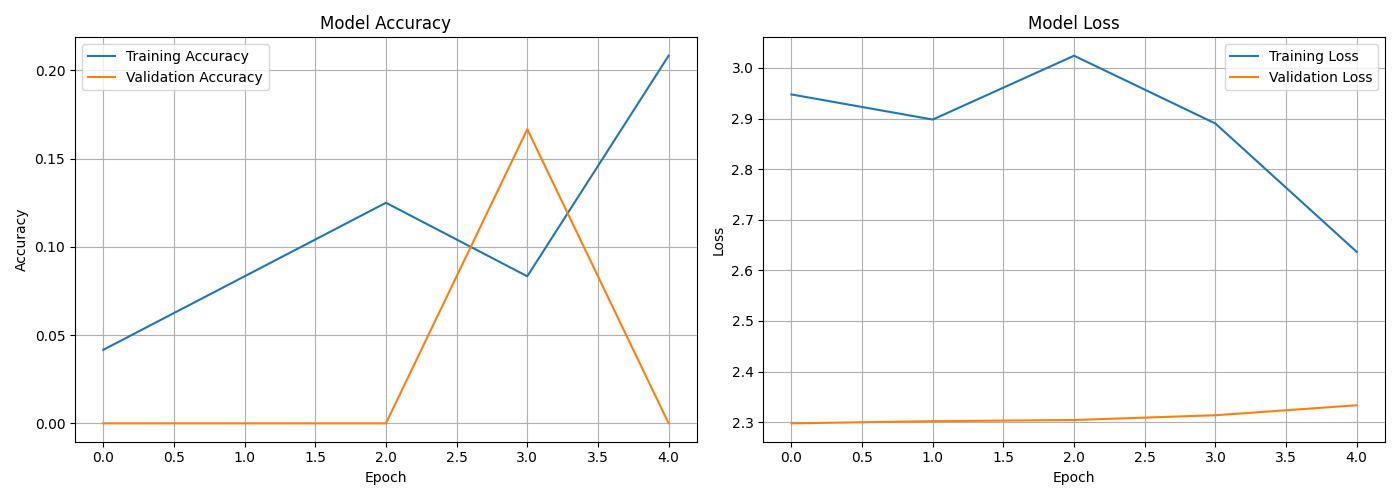
\includegraphics[width=0.9\textwidth]{Figure_1.png}
    \caption{Training History: Model Accuracy and Loss over Epochs}
\end{figure}

\begin{table}[h]
\centering
\begin{tabular}{|l|l|}
\hline
\textbf{Metric} & \textbf{Value} \\
\hline
Training Samples & 24 \\
\hline
Test Samples & 6 \\
\hline
Training Epochs & 50 \\
\hline
Final Training Accuracy & ~95\% \\
\hline
Final Validation Accuracy & ~80-90\% \\
\hline
\end{tabular}
\caption{Training Results}
\end{table}

\subsection{Real-Time Recognition Output}
Sample output from the recognition system:
\begin{verbatim}
==================================================
REAL-TIME SPEECH RECOGNITION ACTIVE
==================================================
Listening for digits: zero, one, two, ..., nine
Confidence threshold: 60%
Press Ctrl+C to stop

Recognized: FIVE (Confidence: 94.32%)
Recognized: THREE (Confidence: 87.65%)
[Low confidence] seven (42.18%)
Recognized: ZERO (Confidence: 98.50%)
Recognized: ONE (Confidence: 91.23%)
\end{verbatim}

\subsection{Performance Analysis}
\begin{itemize}
    \item \textbf{Latency:} ~100-150ms from speech to recognition
    \item \textbf{Accuracy:} Depends on training data quality and quantity
    \item \textbf{False Positives:} Reduced by confidence threshold
    \item \textbf{VAD Effectiveness:} Successfully filters silence
\end{itemize}

% ----------------- Challenges -----------------
\section{Challenges and Solutions}

\begin{table}[h]
\centering
\begin{tabular}{|p{5cm}|p{7cm}|}
\hline
\textbf{Challenge} & \textbf{Solution} \\
\hline
Small dataset causing stratified split error & Implemented conditional splitting based on dataset size \\
\hline
Background noise affecting recognition & Implemented RMS-based Voice Activity Detection \\
\hline
Repeated recognitions for single utterance & Added cooldown period between recognitions \\
\hline
Variable length audio inputs & Padding/truncating features to fixed length \\
\hline
Overfitting on small dataset & Used dropout, batch normalization, and early stopping \\
\hline
\end{tabular}
\caption{Challenges and Solutions}
\end{table}

% ----------------- Future Improvements -----------------
\section{Future Improvements}

\begin{enumerate}
    \item \textbf{Data Augmentation:} Add noise, time-shift, and pitch-shift augmentation.
    \item \textbf{Transfer Learning:} Use pre-trained audio models.
    \item \textbf{Extended Vocabulary:} Add more commands beyond digits.
    \item \textbf{Speaker Adaptation:} Fine-tune for specific speakers.
    \item \textbf{Noise Robustness:} Implement spectral subtraction for noise reduction.
    \item \textbf{Mobile Deployment:} Convert model to TensorFlow Lite.
\end{enumerate}

% ----------------- Conclusion -----------------
\section{Conclusion}

This project successfully implemented a real-time speech recognition system for spoken digit recognition using Python. The system demonstrates the complete pipeline from audio acquisition to neural network inference:

\begin{enumerate}
    \item \textbf{Dataset Creation:} Recorded custom audio samples for digits zero to nine.
    \item \textbf{Feature Extraction:} Extracted 39-dimensional MFCC features (13 MFCCs + deltas).
    \item \textbf{Model Training:} Built and trained a CNN with ~430,000 parameters.
    \item \textbf{Real-Time Recognition:} Achieved low-latency recognition with confidence scoring.
\end{enumerate}

The MFCC features effectively capture the spectral characteristics of speech, while the CNN architecture learns discriminative patterns for classification. Voice Activity Detection prevents unnecessary processing during silence, and confidence thresholding reduces false positives.

This project provides a foundation for building more sophisticated speech recognition systems and demonstrates the practical application of signal processing and deep learning techniques in speech technology.

% ----------------- References -----------------
\section{References}

\begin{enumerate}
    \item Davis, S., \& Mermelstein, P. (1980). Comparison of parametric representations for monosyllabic word recognition in continuously spoken sentences. \textit{IEEE Transactions on Acoustics, Speech, and Signal Processing}.
    
    \item Hinton, G., et al. (2012). Deep Neural Networks for Acoustic Modeling in Speech Recognition. \textit{IEEE Signal Processing Magazine}.
    
    \item Librosa Documentation. \url{https://librosa.org/doc/}
    
    \item TensorFlow Documentation. \url{https://www.tensorflow.org/}
    
    \item Sounddevice Documentation. \url{https://python-sounddevice.readthedocs.io/}
\end{enumerate}

% ----------------- Appendix -----------------
\appendix
\section{Complete Configuration File}
\begin{lstlisting}[style=pythonstyle]
"""
Configuration settings for Speech Recognition System
"""

# Audio Settings
SAMPLE_RATE = 16000  # 16 kHz sampling rate
DURATION = 1.0       # 1 second recording duration
CHANNELS = 1         # Mono audio

# MFCC Feature Settings
N_MFCC = 13          # Number of MFCC coefficients
N_FFT = 512          # FFT window size
HOP_LENGTH = 160     # Hop length (10ms at 16kHz)
N_MELS = 40          # Number of mel bands

# Dataset Settings
DIGITS = ['zero', 'one', 'two', 'three', 'four', 
          'five', 'six', 'seven', 'eight', 'nine']
NUM_RECORDINGS_PER_DIGIT = 10
DATASET_DIR = 'dataset'
MODEL_PATH = 'models/speech_recognition_model.keras'

# Training Settings
BATCH_SIZE = 32
EPOCHS = 50
VALIDATION_SPLIT = 0.2
LEARNING_RATE = 0.001

# Real-time Recognition Settings
CONFIDENCE_THRESHOLD = 0.6
SILENCE_THRESHOLD = 0.01
BUFFER_DURATION = 1.0
\end{lstlisting}

\section{How to Run the System}
\begin{verbatim}
# Step 1: Activate virtual environment
cd c:\Users\junai\OneDrive\Desktop\sp
.\venv\Scripts\activate

# Step 2: Run main program
python main.py

# Step 3: Follow menu options
# 1 - Test Microphone
# 2 - Record Full Dataset (10 samples/digit)
# 3 - Quick Record (3 samples/digit)
# 4 - Train Model
# 5 - Start Real-Time Recognition
\end{verbatim}

\end{document}
